\documentclass{article}


%preamble
%required
%\usepackage{Sweave} %Integrates R code with LaTeX for creating dynamic reports
\usepackage{natbib}%Provides citation and bibliography support
\usepackage{amsmath}%Enhances mathematical typesetting capabilities.
\usepackage{textcomp}%among other things, it allows degrees C to be added
\usepackage{float}%Helps with precise figure placement using the [H] option.
\usepackage[utf8]{inputenc} % allow funny letters in citations 
\usepackage[nottoc]{tocbibind} %should add Re fences to the table of contents?
\usepackage{amsmath} % making nice equations 
\usepackage{listings} % add in stan code
\usepackage{xcolor}
\usepackage{capt-of}%allows me to set a caption for code in appendix 
\usepackage[export]{adjustbox} % adding a box around a map
\usepackage{lineno}
\linenumbers

\usepackage[margin=2cm]{geometry}
\usepackage[most]{tcolorbox}

\newtcolorbox{mytextbox}[1][]{% specify textbox
	sharp corners,
	enhanced,
	colback=white,
	height=15cm,
	attach title to upper,
	#1
}

% recommended! Uncomment the below line and change the path for your computer!
% \SweaveOpts{prefix.string=/Users/Lizzie/Documents/git/teaching/demoSweave/Fig.s/demoFig, eps=FALSE} 
%put your Fig.s in one place! Also, note that here 'Fig.s' is the folder and 'demoFig' is what each 
% Fig. produced will be titled plus its number or label (e.g., demoFig-nqpbetter.pdf')
% make your captioning look better
\usepackage[small]{caption}

\usepackage{xr-hyper} %refer to Fig.s in another document
\usepackage{hyperref}

\setlength{\captionmargin}{30pt}
\setlength{\abovecaptionskip}{0pt}
\setlength{\belowcaptionskip}{10pt}

% optional: muck with spacing
\topmargin -1.5cm        
\oddsidemargin 0.5cm   
\evensidemargin 0.5cm  % same as odd side margin but for left-hand pages
\textwidth 15.59cm
\textheight 21.94cm 
% \renewcommand{\baselinestretch}{1.5} % 1.5 lines between lines
\parindent 0pt		  % sets leading space for paragraphs
% optional: cute, fancy headers
\usepackage{fancyhdr}
\pagestyle{fancy}
%\fancyhead[LO]{Frederik Baumgarten}
%\fancyhead[RO]{Research Proposal}
% more optionals! %

\usepackage{graphicx}
\graphicspath{{/Users/frederik/github/PlantDeterminism/figures/}} % specify the path to your figures directory




\begin{document}
	
	
	\title{Invest now, get paid later? Growth strategies to cope with environmental stress and benefit from extended growing seasons in a future climate %(my favourite)
		
		%dlDec18: Alternate title ideas:
		%Growth determinism/determinacy/habits in plants/woody perennials/trees: Limits and opportunities of species to time growth activities in a future climate. 
		
		%Growth determinacy in temperate trees: investing at the right time to cope with environmental stress and benefit from extended growing seasons in a future climate.
	} 
	
	\date{\today}
	\author{Frederik Baumgarten\textsuperscript{1,2}, Yann Vitasse\textsuperscript{2}, Sally?, Rob?, EM Wolkovich\textsuperscript{1}}
	\maketitle
	
	$^1$ Department of Forest and Conservation, Faculty of Forestry, University of British Columbia, 2424 Main Mall
	Vancouver, BC Canada V6T 1Z4. \\
	
	$^2$  Swiss Federal Institute for Forest, Snow and Landscape Research WSL, Zürcherstr. 111, Birmensdorf 8903, Switzerland\\
	
	Corresponding Author: Frederik Baumgarten; frederik.baumgarten@ubc.ca \\
	Journal: Perspective in Ecology Letters
	
	%Full word count: \\
	%Summary word count: \\
	%Introduction word count: \\
	%Materials and Methods word count: \\
	%Results and figure legends word count: \\
	%Discussion word count: \\
	
	%werwolve: how is tree growth impacted by climate change? 1) by extreme events and 2) by an extended growing season? 
	%baby: better predictions of when environmental factors are influencing growth taking into account the phenological sequence of a species
	%silverbullet: concept of determinism
	
	
\section*{Abstract} %150 words 
	When and how much organisms grow given environmental and other constraints are fundamental questions in biology. For plants their answers are more pressing than ever in order to predict biomass production and carbon sequestration in current and future climates. Increasingly, research has uncovered the relationships between environmental drivers and plant growth, particularly the physiological effects of temperature and moisture extremes. Yet this research has also highlighted that environmental conditions are not enough to predict when a plant is growing. An often-overlooked factor appears to be the phenological sequence---the developmental stages and transitions set by the genetic programming of a plant that manifests in species-specific growth patterns. This internal schedule may be critical to predicting responses to climate change, but is rarely discussed. 
	
	Here, we leverage the concept of (in-)determinacy -- which captures how flexible, or not, plants are in preforming and committing tissue to growth over time -- to propose a new framework for predicting tree responses to climate change. We propose that: 1) determinate growth (expansion of preformed tissue) is an adaptation to predictable climates by allowing temporal escape from critically stressful periods. These species concentrate their primary shoot growth after the last spring frost events and before severe water limitations in summer with ample safety margins.  2) With climate change introducing more frequent, extreme, and irregular stress conditions, species capable of forming new tissue throughout the growing season (indeterminate growth) may recover and compensate from damage more effectively. 3) Additionally, the higher the degree of indeterminacy in a species, the greater its capacity to benefit from extended growing seasons. 
	
	Consequently, the amount of carbon sequestered in future climates may depend not only on abiotic factors such as water availability, temperature extremes, and the length of the growing season, but also on the degree of determinacy set by a species' intrinsic genetic programming.\\
		% : the ability of trees to preform tissue as an investment for next year’s growth that will overwinter in buds vs. a strategy that additionally relies on the continuous activity of the apical meristem throughout the growing season (neo-formed tissue)
		
			\textbf{Keywords}: plant growth, tree phenology, shoot extension, indeterminate growers, carbon sequestration, growing season length, drought, genetic programming, phenotypic plasticity
			\newpage
			
\section*{Introduction}
		Investing the right amount of resources in growth at the right time is of crucial importance to the survival and fitness of any living organism. In some tropical ecosystems a continued production of tissue by trees can be both possible and advantageous; in all other regions, however, strategies that rely on growth from stored reserves and pre-built tissue are common.

	\subsection*{Seasonality of temperature, soil moisture and light}
		The further one travels from the equator towards the poles, the tighter plants are confined to a shrinking `time window of opportunity' set primarily by low temperatures. Below c. 5 °C, metabolic activity slows down to an extent where growth and development cease  \citep{schenkerPhysiologicalMinimumTemperatures2014, rossiCriticalTemperaturesXylogenesis2008, kornerWinterCropGrowth2008}. More importantly, freezing temperatures can cause severe damage to plant tissue if exposed at the wrong time of development, e.g. after leaf unfolding, prior to fruit maturation, or before cold acclimation in fall \citep{sakaiFreezingInjuriesPlants1987c, baumgartenNoRiskNo2023a}. 
		While annual plant species accommodate their entire life cycle within this window, perennial plants are forced to partition their growing phase seasonally, with periods of activity alternating with periods of rest (dormancy). This is referred to as intermittent or rhythmic (as opposed to continuous) growth. \\

		During the active growing season, high temperatures can directly reduce plant growth and development, preventing new growth when species-specific thresholds are exceeded \citep{osullivanThermalLimitsLeaf2017}. High temperatures can also indirectly reduce or stall growth through decreasing soil moisture and thus increasing plant water stress \citep{hsiaoPlantResponsesWater1973, pugnaireConstraintsWaterStress1999, etzoldNumberGrowthDays2021}. Together, these temperature and soil moisture limitations act as environmental filters, narrowing the window of opportunity where potential growth could happen (Figure \ref{fig:fig_1xxx}). Moreover, light can influence growth responses in two ways. First, as the basic energy source (light intensity and quality) driving photosynthesis and consequently source activity. Second, through its relative share to the 24 hours light-dark rhythm (photoperiod), which mediates many physiological processes in a plant's development \citep{wangPlantsDistinguishDifferent2024b}. Both might contribute to the common observation that growth activity peaks around the summer solstice \citep{rossiConifersColdEnvironments2006, etzoldNumberGrowthDays2021}.
	
		
		\subsection*{Internal programming of plants}
		Given our understanding of environmental influences on growth, predicting tree growth in current and future climates might seem straightforward. However, this is not the case, in particular for predictions where climatically favorable growing seasons are being extended \citep{zohnerHowChangesSpring2021}. Here we propose a framework that considers an additional factor: internal growth control---the genetically fixed developmental program that can prevent additional growth of trees \textit{despite} favorable environmental conditions.\\
		
		While plants have evolved many mechanisms to tolerate or avoid such potentially harmful conditions via specialized morphological adaptations, most temperate and boreal species cope with climatically predictable, seasonally fluctuating temperature and moisture regimes by temporally escaping these conditions. This involves timing life history events (phenology) according to a growth and dormancy cycle that balances growth and reproduction with survival for long-lived organisms. Hence, the phenological sequence can impose abrupt switches in resource allocation from vegetative growth to reproduction (flowering, fruit maturation) and storage \citep{stearnsTradeOffsLifeHistoryEvolution1989, chapinEcologyEconomicsStorage1990} that act as internal filters to narrow the window in which growth can occur (Figure \ref{fig:fig_1xxx}).\\
		
		\subsection*{Aim of this perspective/Growth responses in future climates}% any better idea?
		Climate change is extending the growing season length while at the same time increasing the risk for severe drought \citep{haoChangesSeverityCompound2018} and presumably also late spring frost events in many regions worldwide \citep{zohnerLatespringFrostRisk2020}. How are these potential benefits and threats linked to species growth performances? Specifically to their strategy to either preform and/or initiate new shoot tissue from scratch in the current vegetative season (degree of determinacy; see next section)? Which strategy profits most from an extended growing season length and which one can cope better with increased environmental stress? And which one comes with more biomass production and hence C sequestration? The role of primary growth has been widely neglected to help answering these questions, although it sets photosynthetic capacity and therefore to a large degree biomass production \citep{girardPolycyclismFundamentalTree2011}. 
		This perspective aims to revisit traditional research on shoot growth patterns, generalize these concepts across meristem types and place them in the context of climate change. We expect that the mechanisms for internal growth control are key features that can largely influence the response of trees to future climatic conditions.
			
		
								\begin{figure}
								\centering
								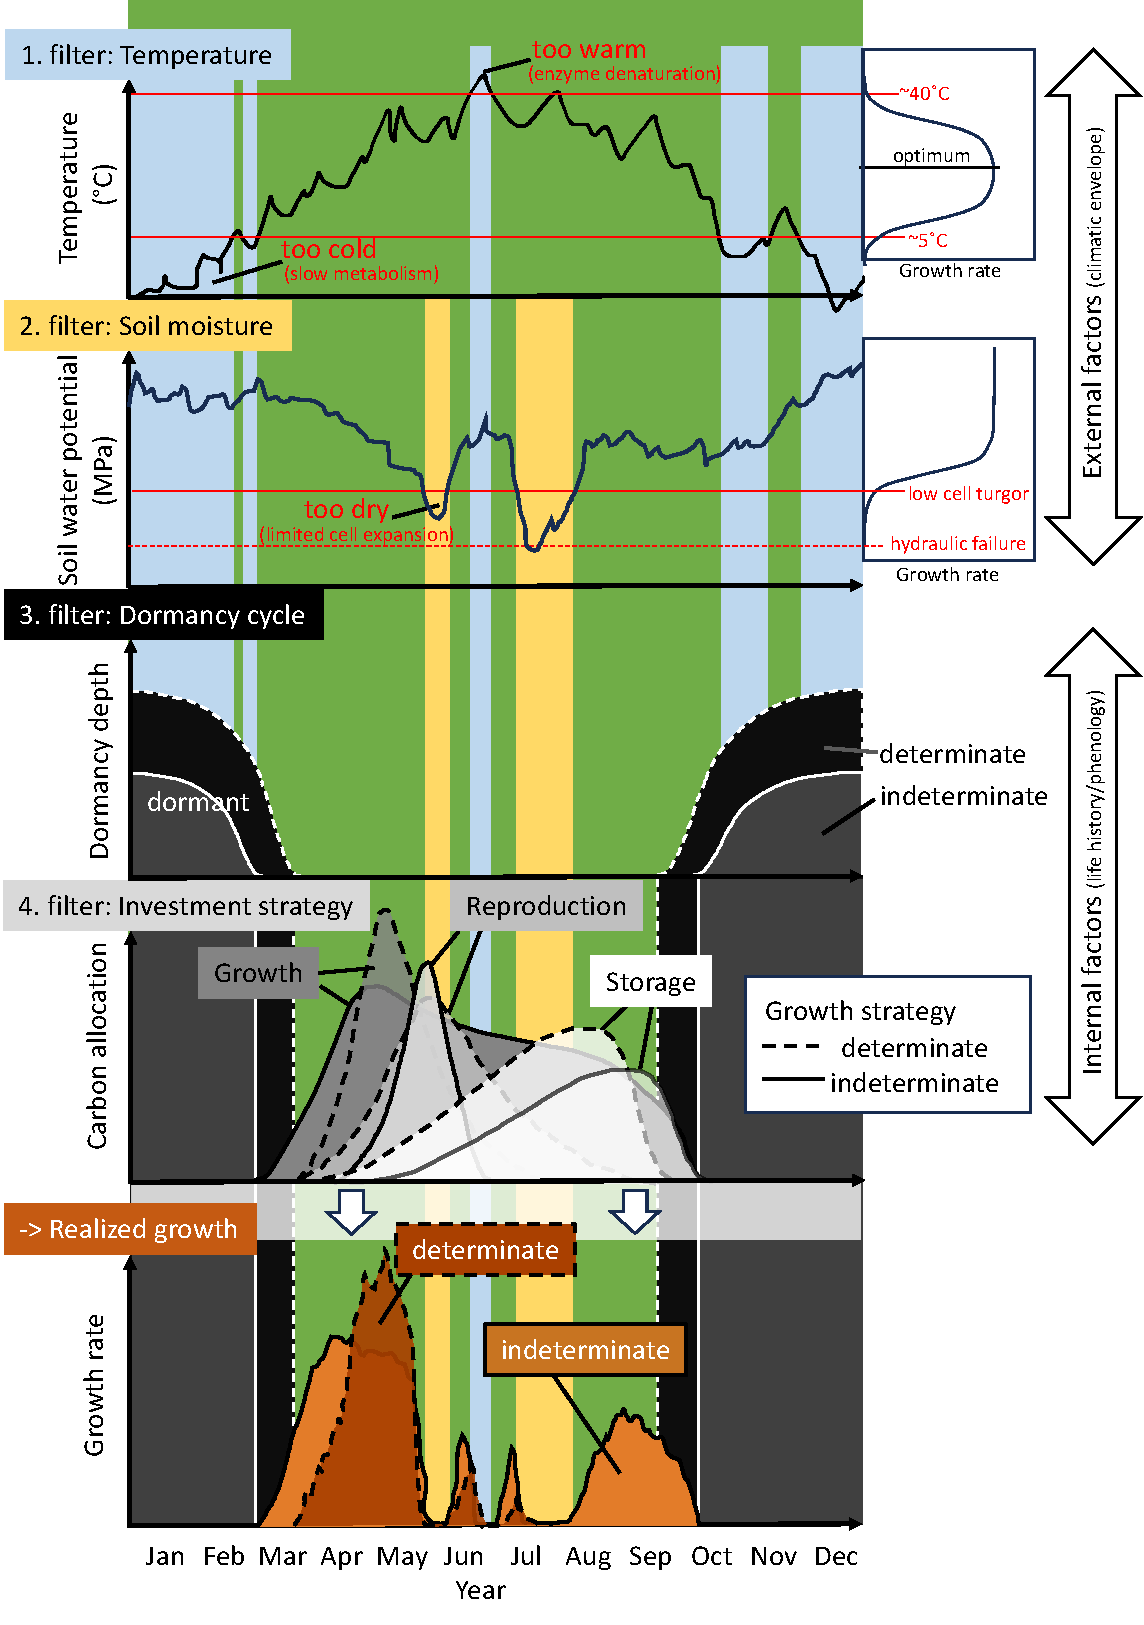
\includegraphics[width=0.9\textwidth]{Fig_1_V6.pdf} 
								\caption{Schematic overview of the possible discrepancy between the potential growing season and the effectively realized vegetative growth. Environmental factors like temperature and soil moisture, exceeding growth-promoting thresholds can be seen as filters that narrow the window of opportunity available for vegetative growth. Potential light and photoperiodic constraints are not shown. The species-specific life history cycle (phenology) can impose another filter by dictating a dormancy cycle and prioritizing developmental processes other than vegetative growth (e.g. flowering, fruit maturation and storage). The degree of (in)determinacy is presented here in two extremes, although we propose to consider this trait as continuous.}
								\label{fig:fig_1xxx}
							\end{figure}

	
\section*{The concept of (in)determinate growth}
	\subsection*{Fixed size or life-long growth} %yann thinks this is too general and we should focus directly on the main definition and on plants
	The topic of growth strategies and habits has a long history in science, spanning the fields of genetics, genomics, physiology and ecology across the animal and plant kingdoms. At its core lays the concept of determinacy---the classification of organisms to either reach a fixed size with adulthood or to continue to grow throughout their lifetime. Like mollusks, fish and reptiles, plants add to their primary bodies as long as they live and are therefore considered `indeterminate growers' \citep{ejsmondHowTimeGrowth2010}. Various terms have emerged to describe this fundamental phenomenon at different spatial and temporal scales, e.g. from a cell to an organism and from a season to a whole lifetime \citep{mcdanielInductionDeterminationDevelopmental1992a, karkachTrajectoriesModelsIndividual2006}. \\

	\subsection*{Full abortion or temporal suspension of the meristem}
	In annual plants, growth ends with the production of flowers to form fruits and seeds: a signal in the apical meristem causes a sudden switch in resource investment from vegetative growth to building a reproductive structure with no point of return, ringing in the end of its life-cycle \citep{poethigPhaseChangeRegulation2003, huijserControlDevelopmentalPhase2011}. An axis that will irreversibly abort meristematic competency and end in a flower or other modified shoot structure is considered `determinate' \citep{barthelemyPlantArchitectureDynamic2007}. In the case of trees, flowers are built on lateral shoots/buds to ensure the continued expansion of the main vegetative structure and the seasonal production of offsprings. However, `determinate growth' also refers to a temporal suspension of the meristem, which leads to a time lag between the formation of tissue and its expansion \citep{kozlowskiSeedGerminationOntogeny2012, halleTropicalTreesForests1978}. 
	
	%yannJuly5: so basically all temperate trees as primordial leaves are formed in the buds before winter. Should we say then that all plants forming buds before the unfavorable season (cold or dry period) are per definition ‘determinate growth’ but the difference occurs during the favorable season where some just expand what has been preformed/planned in the buds, some make new leaves continuously during the growing season after expanding the ones preformed in the buds and some stop after expanding leaves from the buds for a while and make a second flush later (polycyclic growth species)
	
	%robJuly21: To avoid confusion, I think more is needed here to differentiate lateral buds/shoots from terminal buds/shoots, and also to indicate that further discussion mostly relates to the latter.  Even in indeterminate species, most lateral shoots (i.e., the so-called “short” shoots) are determinate whether they hold just leaves or have both leaves and additional tertiary shoots that become flowers.  
	
	%While lateral shoots can be suppressed permanently (so called `short shoots'), terminal shoots commonly follow a such a temporal suspension can be almost permanent in the case of lateral shoots (), 
		
	%Shoot growth patterns do not only tell us something about the plant architecture and the strategy of space exploitation, but may reveal also patterns of the whole-plant dynamic and potential of growth and carbon sequestration.
	
	%unit of extension vs. unit of morphogenesis: Perhaps state somewhere that we commonly only observe the extension pattern while patterns of organogenesis remain hidden. 
	
	%indeterminate growth: functioning of the apical meristems remains intact (but may have periods of rest)
	
	
	\subsection*{Pre- or neo-formation of tissue}
	In their first year of growth, all seedlings have indeterminate growth. After that, many temperate and boreal trees prebuild their new shoot increments in the previous year, overwintering as primordial shoots in hardened buds to be `ready-to-go' when spring arrives. Once the canopy unfolds or extends within a few days to weeks some species suspend further activity of the apical meristem for the rest of the season by internal control mechanism \citep[paradormancy,][]{langEndoParaEcodormancy1987}, often mediated by photoperiod \citep{bohleniusCOFTRegulatory2006a}. Other species, however, continue to produce neoformed leaves and internodes to build on preformed growth, in some cases stretching their growth period into autumn until low temperature forces them to stop. Indeterminate growth can occur either through shoot apical meristems producing new growth without the formation of a bud, or through the formation and subsequent flushing of buds mid-season without a period of dormancy, called second flushing or lammas growth (Figure \ref{fig:fig_2xxx}). \\
	In essence, (in)determinacy in trees as we use it from here on, refers to the ability to:\\
	a) preform tissue in one year as a future investment that is ready to be deployed the following spring with no further primary shoot growth thereafter (determinate strategy)\\
	b) maintain a somewhat constant growth activity (or activity bursts) by forming new tissue during the current growing season (indeterminate strategy)\\

While this concept is often presented as dichotomous \citep{kozlowskiGrowthControlWoody1997, lechowiczWhyTemperateDeciduous1984a}, but see \citealp{kikuzawaLeafSurvivalWoody1983, damascosBudCompositionBranching2005}), with species exhibiting either determinate or indeterminate growth habits, species more likely exist along a gradient with numerous intermediate forms. For example many oaks (\textit{Quercus spp.}) are considered determinate growers, but exhibit a second flush and many species such as Douglas-fir (\textit{Pseudotsuga menziesii}) gradually become more determinate as they mature \citep{borchertConceptJuvenilityWoody1976, heuretOntogeneticTrendsMorphological2006}.\\

								\begin{figure}
								\centering
								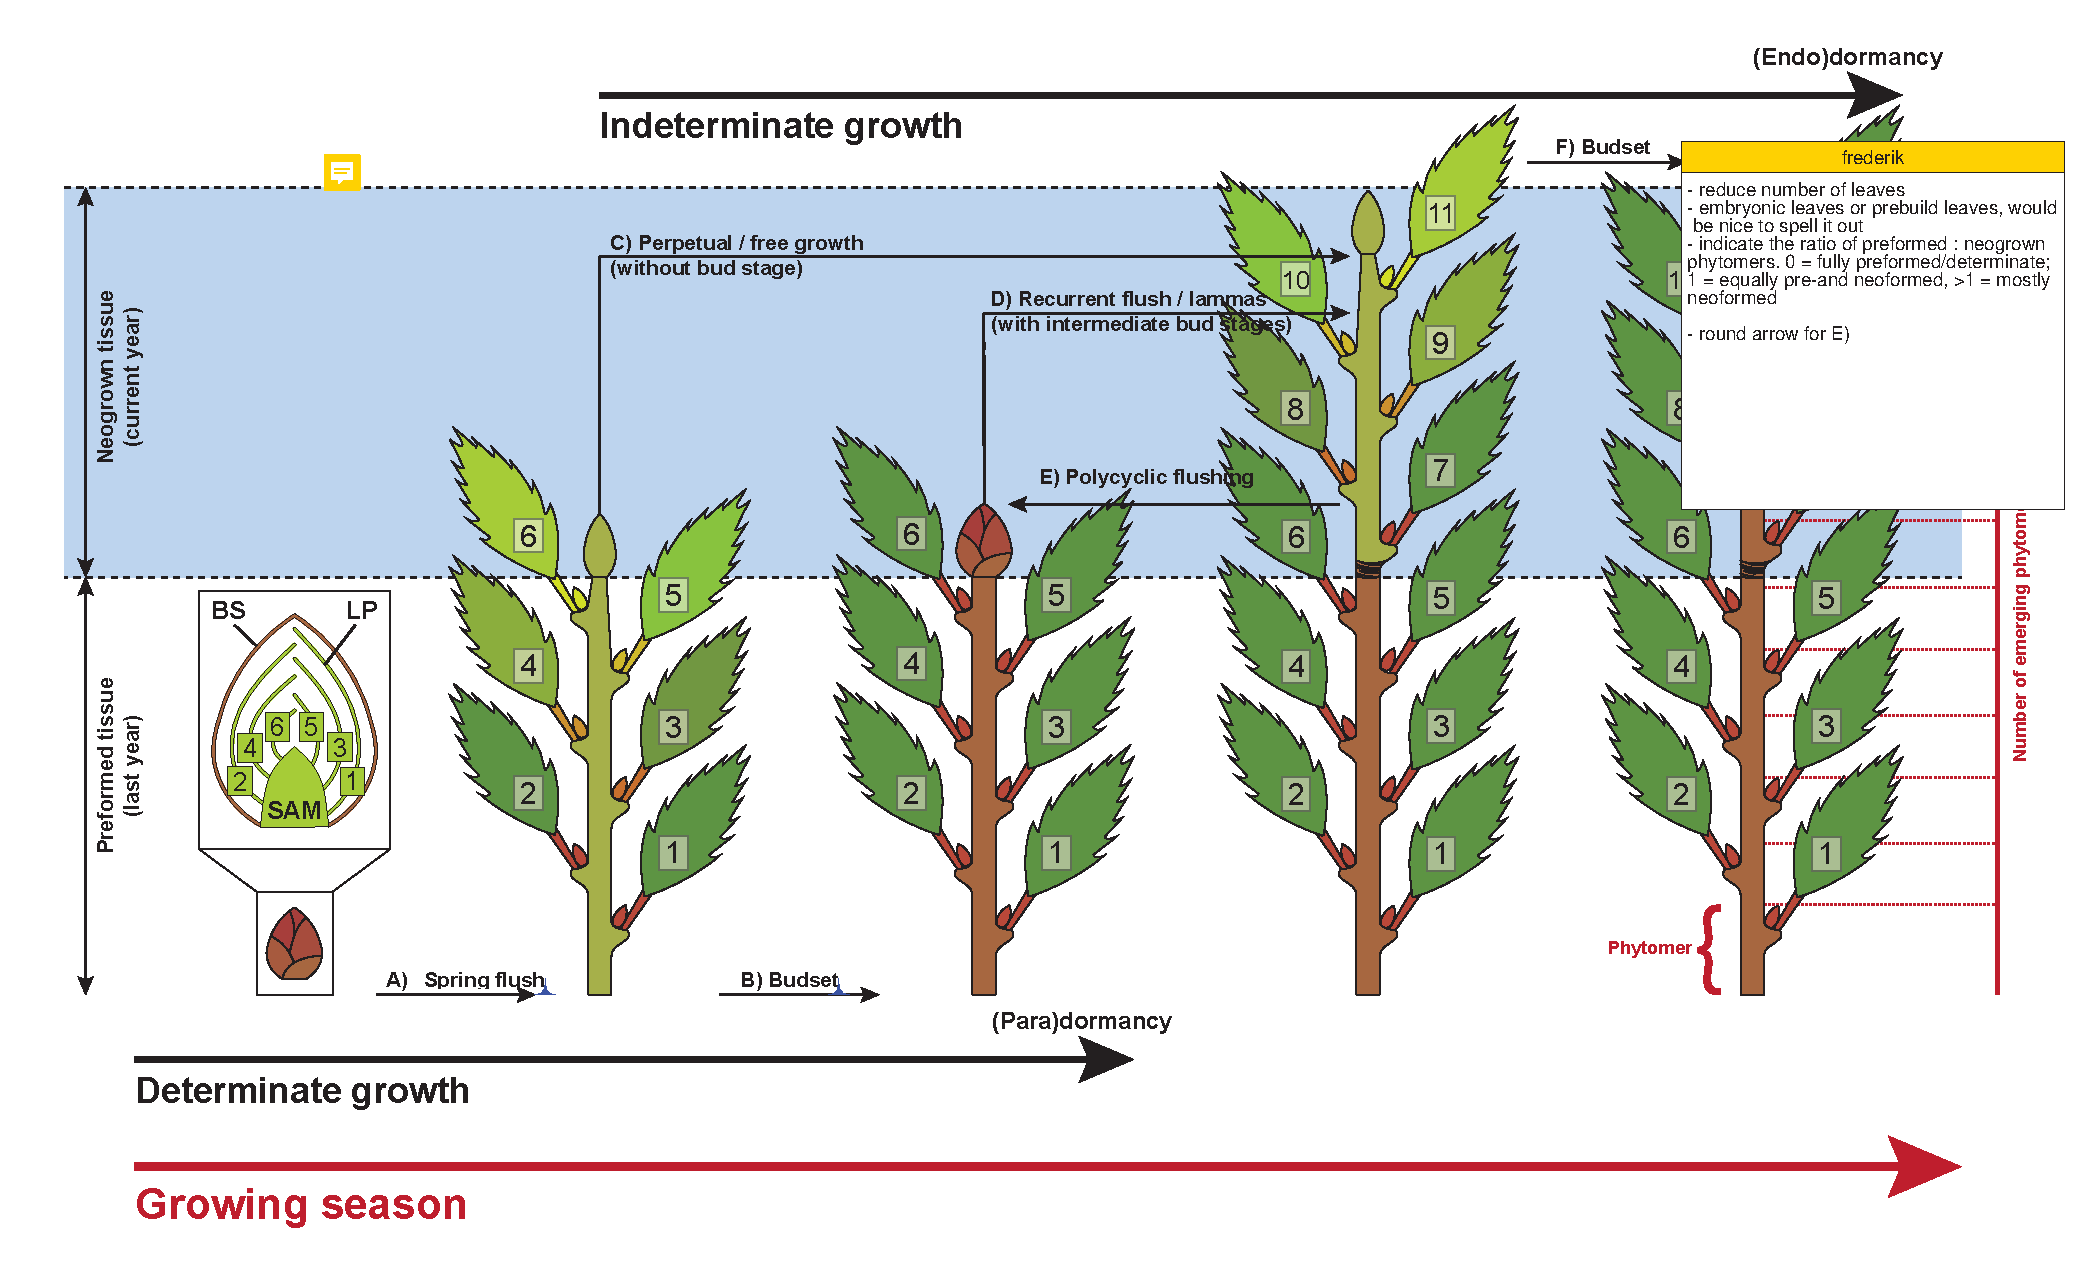
\includegraphics[width=1.1\textwidth]{determinismFigure_FB.pdf} 
								\caption{Determinate and indeterminate growth within one growing season for species producing terminal buds. Commonly all tree species deploy buds during their first (spring) flush from prebuild and overwintering leaf primordia (A). Determinate growing species set buds (B) that are under hormonal suppression to inhibit any further activity of the shoot apical meristem (paradormancy). Indeterminate growing species continue to produce new tissue directly (C) or through one (D) to several (E) intermediate bud stage(s). Finally, most species set their bud (F) and enter full dormancy (endodormancy). Shoot apical meristem (SAM); Bud scale (BS); leaf primordia (LP). The basic unit of a shoot is the phytomer which is composed of a node, a leaf, the axillary bud and an internode.}
								\label{fig:fig_2xxx}
								\end{figure}
								
	\section*{Control mechanisms of (in)determinacy}
	Although a century of studying growth habits and strategies has passed we still have very little understanding of when and why trees exhibit a certain degree of (in)determinacy in their growth strategy. To a large extent this is probably due to the variable environmental conditions within and between years as well as among sites and individuals that complicates the separation of internal from external factors influencing or driving primary shoot growth and for that matter other meristematic activity.
	
	%favourable conditions
	There is indeed evidence that under favorable conditions, particularly under high soil moisture availability throughout the growing season, the time of shoot elongation is extended, e.g. by enabling an additional flush \citep{kayaAdaptiveSignificanceIntermittent1994}. 
	%root:shoot ratio
	Such findings indicate that shoot growth may come to a halt because the demand for water to support an increasing leaf area cannot be met. Hence an imbalance of the root:shoot ratio under a given water status of the plant can suppress shoot growth as was shown experimentally by \citet{borchertSimulationRhythmicTree1973}. By the same mechanism, many species are able to produce new shoots to rebuild the canopy after a considerable loss of leaf area due to herbivory, hail storms or late spring frosts \citep{baumgartenNoRiskNo2023a}. 
	%provenances, adaptation
	However, environmental conditions do not simply alter a species' growth strategy. While a certain plasticity of apical shoot growth has been shown in several species, provenance experiments have also revealed an adaptive component, with the frequency of second flushes increasing in populations of southern origin \citep{rudolphLammasGrowthProlepsis1964, soolanayakanahallyTimingPhotoperiodicCompetency2013a}.
	%photoperiod
	Latitudinal variations in the frequency of second flushes suggest a photoperiodic regulation comparable to that of bud set in poplar species  \citep{soolanayakanahallyTimingPhotoperiodicCompetency2013a}. In fact, bud set, growth cessation and induction of flowering appear to be regulated by the same genes mediated by photoperiod \citep{bohleniusCOFTRegulatory2006a}. Moreover, \citet{wangPlantsDistinguishDifferent2024b} found that plants distinguish between an absolute and photosynthetic-relevant photoperiod to independently control flowering and vegetative growth. 
	Although photoperiod is a promising candidate for regulating growth and development along the seasonal cycle of plants, our knowledge of it is currently based almost exclusively on model organisms, with poplar being the only woody perennial species studied. Hence genetic control mechanisms of (in)determinacy that set the potential of tree growth across species are yet to be discovered. 
	
	%ontogeny as another control mechanism: becoming more conservative and determinate with age	
	
										
	\subsection*{Evolution of (In)determinacy}
	Understanding how universally tissues within species are formed determinately or indeterminately could provide insight into the evolution of this trait, which could be aided by cross-species analyses. Both growth forms seem to occur across most species of the same genera or clade and hence, appear to have evolved repeatedly in different groups (Figure \ref{fig:fig_4xxx}), making it difficult to speculate on which strategy is ancestral \citep[but see][]{hariharanIndeterminateGrowthCould2016} and how rapidly (in)determinacy can evolve. As data on which species are determinate or indeterminate accumulates, such analyses could potentially provide rapid insights into this, and also aid forecasting for unsampled species. Assigning species as determinate or indeterminate, however, may not be useful if the trait is actually better considered as continuous. \\

	But what are the fundamental trade-offs associated with adopting either strategy? In most temperate and boreal ecosystems both growth strategies are successful and co-occur in communities. The enhanced growth potential of indeterminate species allows to easily outgrow competing species. Faster growth, however, might lead as well to faster turnovers and a shorter life spans \citep{brienenForestCarbonSink2020b, milletRelationshipArchitectureSuccessional1999}. Not surprisingly, indeterminate growing species are often found to be early successional ones \citep{marksRelationExtensionGrowth1975, boojhGrowthStrategyTrees1982}, indicating a niche separation of these two growth forms. 
	%section from Sally:
	Moreover, indeterminate growth provides a mechanism for phenotypic plasticity in growth in response to current conditions. Determinate growth can also result in phenotypic plasticity, but will be affected to a greater extent by conditions in the previous year during bud formation. Current conditions during bud break and shoot elongation can also affect internode length to some extent, but phenotypic plasticity for primary shoot growth is likely to be lower in more determinate species. Determinate species might therefore be expected to have a greater degree of local adaptation of populations to historic, local climates, and less phenotypic plasticity than indeterminate species \citep{leitesForestTreeSpecies2023}. For example, western larch (\textit{Larix occidentalis}) achieves much of its primary shoot growth from indeterminate growth %(a combination of lammas and neoformed shoot growth), 
	and is less locally adapted than the sympatric species Douglas-fir, which is more determinate (Roskilly and Aitken, in press).\\

	As climate changes the question arises which growth strategy will be more successful in the future.

								
%	\begin{mytextbox}[]
	%	\subsection*{Box 1: Definitions)}
	%	\textbf{Growth habit}: The genetic tendency of a plant to form a characteristic habitus (shape, height, form) with a particular branching and growth pattern. \\
%		\textbf{determinate growth}: a growth pattern characterized to stop at a predefined size. Commonly, the apical bud culminates in an inflorescence, halting the production of any additional leaves or buds. In trees this terms specifies the short duration of extension growth in spring with no further activity of the apical meristem.\\
		%\textbf{indeterminate growth}: a growth pattern characterized by continuous growth (leaves, buds or flowers) throughout their life or as long as condition remain favourable. This is possible because the apical meristems always remain vegetative and flowers are restricted to lateral meristems. In trees this refers to the continuous shoot elongation throughout the growing season.\\
		%\textbf{Neogrowth}: Growth that occurs on top of preformed tissue due to the more or less continuous activity of the shoot apical meristem. Several forms occur depending on whether growth occurs continuously or in bursts.\\
		%\textbf{Perpetual/Continuous/free/sustained growth}: the constant production of new tissue without interruptions of bud stages.\\
		%\textbf{Polycyclic flushing:} successive bursts of shoot growth interrupted by bud set and a resting phase within the same vegetative period   \\
		%\textbf{Second flush:} Growth form of species in which one additional cohort of buds is build and deployed during the current growing season. In the German literature this is often termed ‘Johannitrieb’ since the flush often occurs around the summer solstice. Also ‘lammas growth’ is a common term for an additional flush.\\
		%prolepsis = a rhythmic branching process, during which a bud underwent a dormancy phase and subsequently extends into a branch. Determinate species have only proleptic branches.
		%syllepsis = a continuous branching process, during which an incomplete axillary bud without a resting phase extends into a branch. Indeterminate species have both proleptic and sylleptic branches. 
	%\end{mytextbox}

	
\section*{The role of (in)determinacy with climate change} %Yann: I don’t like the title it’s more how climate change may affect differently the species upon their degree of determinacy 

Spring warming has advanced the onset of leaf emergence by up to a month compared to pre-industrial times \citep{vitasseGreatAccelerationPlant2022b}. In contrast, autumn phenology of growth and leaf senescence has not been delayed to the extent one might predict from environmental conditions \citep{zaniIncreasedGrowingseasonProductivity2020b, zohnerEffectClimateWarming2023}. In fact, the phenological sequence is observed to shift more as a whole towards spring with warming \citep{keenanTimingAutumnSenescence2015b}, not necessarily leading to increased biomass production during longer growing seasons \citep{zaniIncreasedGrowingseasonProductivity2020b}. We hypothesize that only determinate growing species shift their growth in such a way with minimal changes in overall productivity. In contrast, indeterminate growing species are able to extend their growing period in both directions, potentially leading to an increased productivity in a future climate (Figure \ref{fig:fig_4xxx}). \\
%Yann: But we should keep in mind that if indeterminate growth strategies is mainly found in early successional species, climate change will not really change the cards, perhaps just accelerate the transition phase between early and late successional species…

The flexible growth strategies of indeterminate species that help them exploit longer seasons could also increase their exposure to extreme climatic events. Deciduous indeterminate species are often among the first to leaf-out and among the last to shed their leaves \citep{marksRelationExtensionGrowth1975, boojhGrowthStrategyTrees1982}---occasionally as a result of first freezing events in autumn. In addition, a substantial part of their growth period falls into periods of summer with increased risk of drought (Figure \ref{fig:fig_4xxx}). Therefore, we hypothesize that the conservative strategy of determinate growth largely escapes unfavorable growing conditions by growing between the last spring frost and the increasing water shortages in summer, with relatively ample safety margins. As a consequence productivity shows little between year variation and will largely remain constant in a future climate. However, once hit by an extreme event, determinate growing species might not recover easily. Even if leaves are shed to prevent further damage, the loss of the canopy, which is rarely replaced after the summer in determinate species, will prevent replenishment of the reserve pools and ultimately reduce fitness. In contrast, the flexible growth schedule of indeterminately growing species may allow to 1) produce tissue better adapted to harsh environmental conditions as it is formed in the current season and 2) catch up and compensate later in the season by another productivity boost. Taking advantage of a `second growing season' after summer drought was indeed shown for pines in the Mediterranean` climate through polycyclic flushing---a form of indeterminate growth \citep[Figure \ref{fig:fig_2xxx}]{girardPolycyclismFundamentalTree2011}. \\

We argue that new opportunities and challenges for trees with climate change will increasingly disrupt their phenological cycle, favoring species and genotypes that are more plastic in rearranging their activities by resuming growth, reproduction and/or storage filling later in the year, thereby recovering from and compensating for some stress-induced damages and losses. Future climate will therefore likely intensify the competition among co-occurring species and might re-assemble forest communities increasingly composed of species adopting an indeterminate growth strategy.
	
	
								\begin{figure}
								\centering
								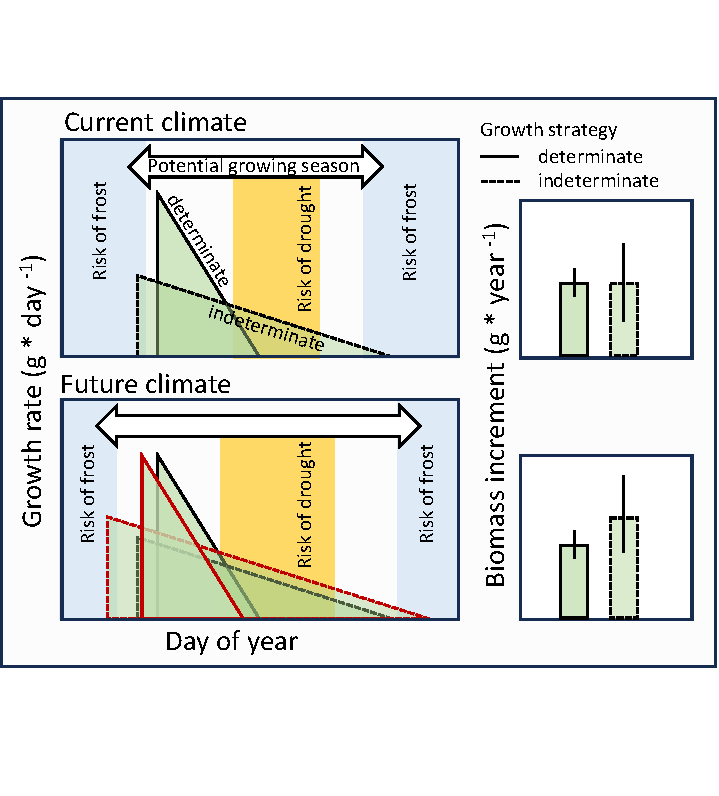
\includegraphics[width=0.9\textwidth]{Fig_4_V1.pdf} 
								\caption{Hypothesized predictions of growth rates under current and future climate for determinate and indeterminate growing species. Note that the indeterminate strategy is more exposed to the risk of frost and drought events while the determinate strategy condenses most growth within a rather safe period. In the current climate the indeterminate strategy is in balance with benefiting from the full climatic growing season in some years with some drawback in other years, resulting in the same mean yearly biomass increment, but with a higher variation; right box). In a future climate the indeterminate strategy might benefit from longer growing seasons, resulting in an overall higher mean annual biomass increment compared to determinate growers, but this will be dependent on the severity of drought.}
								\label{fig:fig_4xxx}
							\end{figure}
	\pagebreak
\section*{Future directions}
We argue that incorporating plant determinacy into models of forest dynamics could provide better answers to major questions of climate change responses and . . .. The impacts of climatic extremes and longer growing seasons on primary and secondary growth, and therefore carbon sequestration, may depend on the ratio of indeterminate to determinate growing species in a forest community. Better understanding these two strategies will also help to reveal the potentials and limits of trees to adapt in a future climate, and may inform species or provenance choices for reforestation or restoration.

Understanding how much (in)determinacy allows trees to escape periods of increased risk of environmental stress while being versatile enough to resume metabolic activities to repair damaged structures, restore reserves and eventually compensate for previous losses during the same season is an important knowledge gap. Assessing the trade-off between buffering or avoiding extreme events and exploiting a longer growing season will likely contribute to our understanding of how forest communities will survive and assemble over the course of this century.\\

Going forward, we need to characterize the plasticity of and mechanisms of indeterminate growth under different environmental conditions, the genetic programming of a species, and to what extend the latter prioritizes the former. This research is needed across species and populations and should involve disciplines ranging from genetics and genomics to physiology and ecology. Moreover, we need to understand how much indeterminate growth will impact carbon sequestration, which will depend on how universal the concept of (in)determinacy holds across tissue and meristem types.

\subsection*{(In)determinacy beyond leaf tissue} 
Although (in)determinate growth is mainly associated with the activity of the shoot apical meristem, a similar pattern or concept might be found in the cambium as well to ensure a timely switch from earlywood to latewood production, or from vegetative growth to reproductive and storage investments. Cambial initial cells produce daughter cells that subsequently divide to produce several cohorts of precursor cells, with cell differentiation and maturation being completed at a later stage \citep{valdovinos-ayalaSeasonalPatternsIncreases2022}. Hence the number of initial cell divisions largely determines the amount of total xylem produced \citep{lupiXylemPhenologyWood2010}. Primary growth influences the overall secondary growth of an individual through auxin production?. The low predictive power to estimate the end of wood formation in autumn reported by several studies \citep{buttoComparingCellDynamics2020} indeed points to a mechanism that stem growth in many tree species ceases despite of ongoing favorable conditions and a green canopy \citep{arendStemGrowthPhenology2024}.\\

Regarding below-ground meristems, roots seem to follow a much more opportunistic strategy with indeterminate growth potentially occurring throughout the year, with peaks in spring and again late in the growing season. Warming experiments using rhizotrons have shown that roots can even grow mid-winter if temperatures allow \citep{lyfordControlledGrowthForest1966}, suggesting that roots do not enter a state of dormancy \citep{radvilleRootPhenologyChanging2016}. To what extent asynchronies between above and below-ground meristems occur as a result of different temperatures experienced, root:shoot imbalances or genetically fixed investment strategies remains unresolved \citep{abramoffAreBelowgroundPhenology2015, makotoSynchronousAsynchronousRoot2020}.\\

 Future studies should therefore link the temporal dynamics of primary (apical and root) and secondary (cambial) meristems. Correlating annual tree rings with shoot increments could reveal such a common pattern, if accounting for when inter-annual shoot segments (phytomers) were produced, e.g. separating preformed from neo-grown tissue (REF Günter?). Revealing the patterns of when different meristems are active will likely contribute to a theoretical framework of temporal carbon allocation dynamics.
 
 %Sally:
 %Seems like there should be a paragraph about deciduous versus evergreen species, and the potential differences in outcomes of (in)determinacy. Of course, evergreen species are not as reliant on the new leaf area produced in a single year – would that lead to a prediction of greater determinacy?

							\begin{figure}
							\centering
							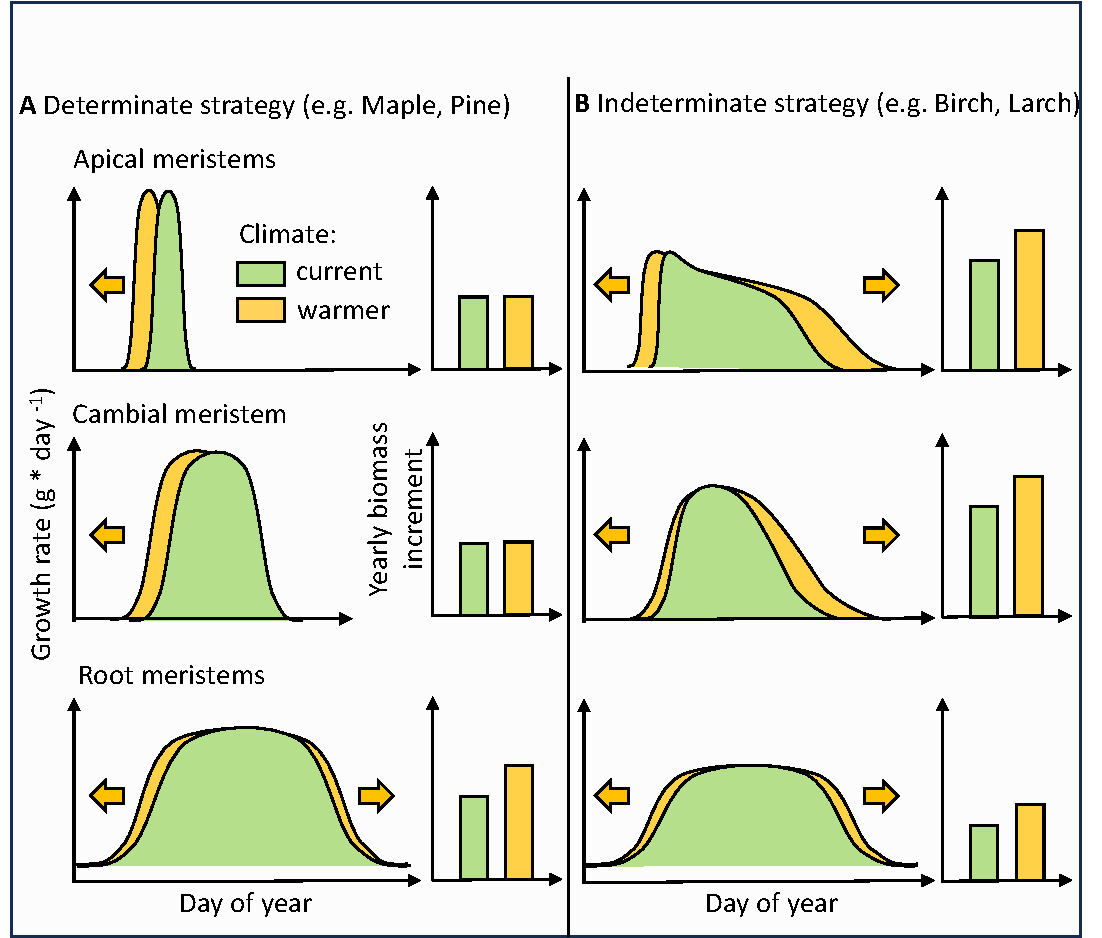
\includegraphics[width=0.9\textwidth]{Fig_3_V3.pdf} 
							\caption{Hypothesized predictions of growth rates for the three major meristem (apical, cambium and root) classes of trees under current and warmer climates following an extreme determinate (A) and indeterminate (B) growth strategy. The area under the curve is summarized as yearly biomass increment in the respective bar-plot. Arrows indicate the shift of growth phenology under warmer climate conditions. Root meristems appear to be purely temperature opportunistic for both strategies, even growing during warm winter spells. The indicated genera were observed to showcase the illustrated trends. The responses of these two contrasting growth strategies might apply not only to different tree species but also within a population (e.g. along environmental gradients) and even within an individual as it transitions from the juvenile to the adult stage (ontogeny).}
							\label{fig:fig_3xxx}
						\end{figure}

	
	\subsection*{Metrics of (In)determinacy} % probably put into a box
	To address these questions we need better metrics to quantify the degree of determinacy, moving beyond a dichotomous classification system. We propose several metrics from best to acceptable, with increasing spatial scale: \\
	
	(1) The ratio of the number of leaves at the end of the season to the initial number of leaf primordia in buds at the start of the season provides a good measure of (in)determinacy. Values above one indicate an increasing degree of indeterminate growth. Although this metric was already described over a century ago by \citet{mooreStudyWinterBuds1909}, its application has been limited to few studies exploring specific regions only \citep{damascosBudCompositionBranching2005, kikuzawaLeafSurvivalWoody1983, guedonRelativeExtentsPreformation2006}. Moreover, to reveal the endogenous potential of indeterminate growth, individuals have to be grown under constant favorable conditions (e.g. unlimited soil moisture).\\
	
	(2) Direct measures of shoot elongation (height increments) and/or xylogenesis (micro-cores) at high temporal resolution (e.g. bi-weekly) to assess the temporal dynamics of apical and cambial activity. Especially wood anatomical observations ensure the distinction of cell formation and their subsequent enlargement and development REFS\\
	
	(3) As a proxy for the above, dendrometers provide insights of xylem and phloem formation at high temporal resolution. Although obtained measurements are a mixture of several processes, it allows to identify the tree water deficits and related growth reductions \cite{etzoldNumberGrowthDays2021, zweifelWhyTreesGrow2021}. \\
	
	(4) Using observations of 'second flushes' in large databases (e.g. US national forest network). \\%@Lizzie: any references here and examples/specifics of how to use it?
	
	(5) Patterns and fluctuations of canopy growth can be detected from drones or satellites using LiDAR or various spectral techniques. The temporal trend of canopy greenness over the growing season can reveal investment strategies integrated across entire ecosystems and vast areas. As a recent example, \citet{mengConsistentTimeAllocation2024} found that time allocation between vegetation green-up (from start of the growing season to its peak) and vegetation senescence (between peak and end of season) remained constant despite substantial differences in growing season lengths and degree of warming in temperate ecosystems across the northern hemisphere.  %Could be also a section "Evidence for internal growth control" 

	%number of  growth days under favourable conditions for both total growth and neogrowth
	
	%

	
\section*{Acknowledgments}
	This text emerged from a grant of the Swiss National Foundation to F.B. (grant number P500PB\textunderscore 210943). We thank J. Ngo for designing figure 2 and XXXX
	
	

	
	\pagebreak
	

	\newpage
\section*{stuff I did't find place yet}

Deciduous tree species have a higher number of leaf primordia inside their buds than evergreen species in the Cerrado (Brazil). 
	
If experiments are conducted in conditions with unlimited soil moisture and under similar temperature regimes, then the dynamics of growth responses can be comparable among species and reveal their potential in deploying indeterminate growth. Under natural conditions with common soil moisture and associated turgor limitations it is currently hard to tell if trees cease growth because of a response to the environment or because of switches in resource allocation. 
 
 Even in grasslands an earlier onset of growth is associated with an earlier stop under climate warming \cite{mohlGrowthAlpineGrassland2022a}
	
	
	must include: 
	
	\cite{iwasaOptimalGrowthSchedule1989}
	
	
	
	Shoot growth patterns do not only tell us something about the plant architecture and the strategy of space exploitation, but may reveal also patterns of the whole-plant dynamic and potential of growth and carbon sequestration.
	
	unit of extension vs. unit of morphogenesis: Perhaps state somewhere that we commonly only observe the extension pattern while patterns of organogenesis remain hidden. 
	
	\citep{verduEvolutionaryCorrelationsPolycyclic2007}: polycylcic flushing in acer might be associated to maximize the light capture in the understory
	ontogenetic changes towards monocyclic growth might reflect the urge for light in the early life phase
	
	 \citep{wuPhenotypicPlasticitySylleptic2001}: proleptic and sylleptic branching. great reference for phenotypic plasticity and how sylleptic growth (a form of indeterminate growth) might be beneficial more stressful/unpredictable climates
	
	\newpage
	
	\bibliography{refs_determinism}
	\bibliographystyle{ecolett}
	
	
	
\end{document}






